\documentclass{ximera}

\newcommand{\RR}{\mathbb R}
\renewcommand{\d}{\,d}
\newcommand{\dd}[2][]{\frac{d #1}{d #2}}
\renewcommand{\l}{\ell}
\newcommand{\ddx}{\frac{d}{dx}}
\newcommand{\dfn}{\textbf}
\newcommand{\eval}[1]{\bigg[ #1 \bigg]}

\colorlet{textColor}{black} 
\colorlet{background}{white}
\colorlet{penColor}{blue!50!black} % Color of a curve in a plot
\colorlet{penColor2}{red!50!black}% Color of a curve in a plot
\colorlet{penColor3}{red!50!blue} % Color of a curve in a plot
\colorlet{penColor4}{green!50!black} % Color of a curve in a plot
\colorlet{penColor5}{orange!80!black} % Color of a curve in a plot
\colorlet{fill1}{blue!50!black!20} % Color of fill in a plot
\colorlet{fill2}{blue!10} % Color of fill in a plot
\colorlet{fillp}{fill1} % Color of positive area
\colorlet{filln}{red!50!black!20} % Color of negative area
\colorlet{gridColor}{gray!50} % Color of grid in a plot

%% makes a snazzy t-chart for evaluating functions
\newenvironment{tchart}{\rowcolors{2}{}{background!90!textColor}\array}{\endarray}


\outcome{}

\newcommand{\RS}{r^s}

\title[Break-Ground:]{Limits and velocity}

\begin{document}
\begin{abstract}
Here we see a dialogue where two young mathematicians discuss limits
and instantaneous velocity.
\end{abstract}

\maketitle

\newcommand{\again}[2]{X^Y+#1+#2}

Check out this dialogue between $\RS$ two calculus students (based on a true
story):

And then $\again{12}{33}$

\begin{dialogue}
\item[Devyn] Hey Riley, I've been thinking about limits.
\item[Riley] That is awesome.
\item[Devyn] I know! You know limits remind me of something\dots
  How a GPS or a phone computes velocity!
\item[Riley] Huh. To compute velocity from position look at
  \[
  \frac{\text{change in position}}{\text{change in time}}
  \]
\item[Devyn] And then we study this as the change in time gets closer
  and closer to zero.
\item[Riley] Just like with limits at zero, we can study something by
  looking \textbf{near} a point, but \textbf{not exactly at} a point.
\item[Devyn] O.M.G.\ Life's a rich tapestry.
\item[Riley] Poet, you know it.
\end{dialogue}

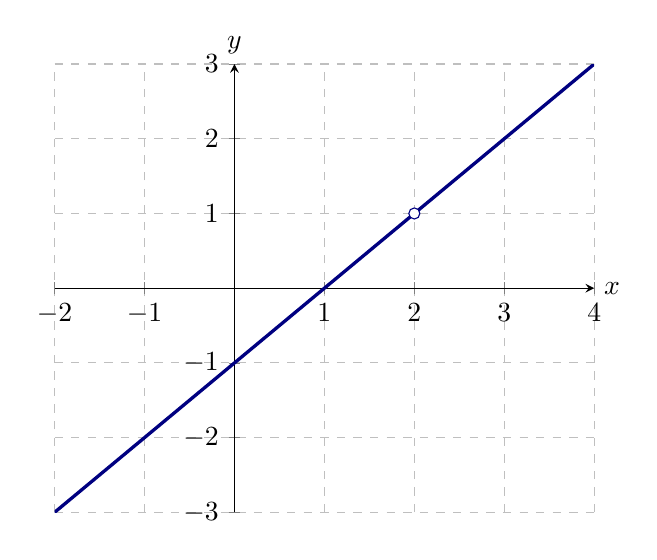
\begin{tikzpicture}
	\begin{axis}[
            domain=-2:4,
            axis lines =middle, xlabel=$x$, ylabel=$y$,
            every axis y label/.style={at=(current axis.above origin),anchor=south},
            every axis x label/.style={at=(current axis.right of origin),anchor=west},
            grid=both,
            grid style={dashed, gridColor},
            xtick={-2,...,4},
            ytick={-3,...,3},
          ]
	  \addplot [very thick, penColor, smooth] {x-1};
          \addplot[color=penColor,fill=background,only marks,mark=*] coordinates{(2,1)};  %% open hole
        \end{axis}
\end{tikzpicture}

Suppose you take a road trip from Columbus Ohio to Urbana-Champaign
Illinois. Moreover, suppose your position is modeled by
\[
s(t) = 36t^2 -4.8t^3 \qquad\text{(miles West of Columbus)} %% note the model is wrong
\]
where $t$ is measured in hours and runs from $0$ to $5$ hours. 

\begin{problem}
Choose a fraction like 
$$
R = \frac{\answer{19}}{\answer{17}}
$$
so that $R^2 \approx 2$.  There's so many possible answers.
\end{problem}

\begin{problem}
Choose another fraction like 
$r = \frac{\answer{1}}{\answer{2}}$
so that $r = 0.5$.  Pick the one I'm thinking of.
\end{problem}

\begin{problem}
Choose a third fraction like 
\[
R = \frac{\answer{20}}{\answer{19}}
\]
so that $R^2 \approx 2$.  There's so many possible answers.
\end{problem}

\begin{problem}\label{problem:whee}
  Set $r=3\cdot t$. Now $P(t) = 2\cdot \pi\cdot 3\cdot t$. What is
  $P'(t)$ when $r=15$?
  \begin{prompt}
    $P'(t)=\answer{2 \pi 3}$
  \end{prompt}
\end{problem}

\begin{problem}
  \label{problem:average-velocity}
  \begin{hint}
    Remember, 
    \[
    \text{change in distance} = \text{rate}\cdot\text{change in time}.
    \]
  \end{hint}
  \begin{hint}
    So, 
    \[
    \frac{\Delta\text{distance}}{\Delta\text{time}} = \text{rate}.
    \]
  \end{hint}
  \begin{hint}
    So, 
    \[
    \frac{\Delta\text{distance}}{\Delta\text{time}} = \frac{300}{5}.
    \]
  \end{hint}
  The average velocity is $\answer[given]{60}$ miles per hour.
\end{problem}

How are you liking this so far?
\begin{freeResponse}
FREE!DOM1
\end{freeResponse}

\begin{problem}
Suppose $f(x)$ is a quadratic polynomial 
\[
f(x) = \answer{2}x^2 + \answer{4}x + \answer{1}.
\]
Make sure that $f(0) = 1$ and $f(1) = 7$ and $f(2) = 17$.
\end{problem}

\begin{problem}
  Use a calculator to estimate the instantaneous velocity at $t=2$.
  \begin{hint}
    Remember, 
    \[
    \text{change in distance} = \text{rate}\cdot\text{change in time}.
    \]
  \end{hint}
  \begin{hint}
    So, 
    \[
    \frac{\Delta\text{distance}}{\Delta\text{time}} = \text{rate}.
    \]
  \end{hint}
  \begin{hint}
    Compute
    \[
    \frac{36(2+\Delta t)^2 -4.8(2+\Delta t)^3 -\left(36\cdot 2^2 -4.8\cdot 2^3\right) }{\Delta t}
    \]
    for smaller, and smaller values of $\Delta t$.
  \end{hint}
  \begin{prompt}
    The instantaneous velocity, (rounded to the nearest tenth) is $\answer{86.4}$ miles per hour.
  \end{prompt}
\end{problem}


\begin{problem}
  Considering the work above, when we want to compute instantaneous
  velocity, we need to compute
  \[
  \frac{\text{change in position}}{\text{change in time}}
  \]
  when (choose all that apply):
  \begin{multipleChoice}
    \choice{The ``change in time'' $2x$ is zero.}
    \choice{The ``change in time'' $\sqrt{x}$ is near zero.}
    \choice[correct]{The ``change in time'' is gets closer and closer to zero.}
    \choice{The ``change in time'' approaches WROPNG.}
    \choice{The ``change in time'' which is $$\frac{1}{2}$$ goes to NOT COERRECT.}
  \end{multipleChoice}
\end{problem}


Computing average velocities for smaller, and smaller, values of
$\Delta t$ as we did above is tedious. Nevertheless, this is exactly
how a GPS determines velocity from position! On the other hand, we are
human beings and have better things to do than just compute all day
long. What would really help us out is a formula.

What could we do better?
\begin{freeResponse}
Here's some sort of free response.
\end{freeResponse}

\end{document}
